\documentclass[11pt,oneside]{book}

% \usepackage[margin=1.75in]{geometry}
\usepackage{graphicx}
\usepackage{caption}
\usepackage{subcaption}
\usepackage{amsmath}
\usepackage{mathrsfs}
\usepackage{nicefrac} %package for nice fractions in exponents
\usepackage{esint} %package for cauchy principal value integral \fint
\usepackage{cancel} %package to strike out maths
\usepackage[colorlinks,bookmarks,bookmarksnumbered,allcolors=blue]{hyperref}
%\usepackage[caption=false,justification=raggedright,singlelinecheck=false]{subfig} %Note Judd swapped this for the caption/subcaption packages and updated the other .tex files so that they have the right syntax. The reason is he couldn't figure out how to use subfig to do a 2x2 sub figure like that in the airfoilparams document.
\usepackage{booktabs} % better tables
\usepackage[capitalise]{cleveref}
\usepackage{floatrow}
\floatsetup[table]{capposition=top}
\usepackage{listings}
\usepackage[usenames,dvipsnames]{xcolor} 
\usepackage{pgf,tikz,pgfplots}
\usetikzlibrary{arrows.meta}
\usepackage{algpseudocode}
\usepackage{algorithm}
\usepackage{appendix}

\graphicspath{{figures/}}

% --- chapter author -----
\makeatletter
\newcommand{\chapterauthor}[1]{%
  {\parindent0pt\vspace*{-25pt}%
  \linespread{1.1}\large\scshape#1%
  \par\nobreak\vspace*{35pt}
  }
  \@afterheading%
}
\makeatother

% % ---- header ----
% \usepackage{fancyhdr}
% \pagestyle{fancy}
% \fancyhf{}
% \fancyhead[L]{\the\year\ BYU FLOW Lab}
% \fancyhead[R]{\thepage}

%--- Bibiliography Styling---
\usepackage{etoolbox}
\patchcmd{\thebibliography}
{\chapter*}
{\section*}
{}
{}
\renewcommand{\bibname}{References}


%%
%% Julia definition (c) 2014 Jubobs
%%
\lstdefinelanguage{Julia}%
{morekeywords={abstract,break,case,catch,const,continue,do,else,elseif,%
		end,export,false,for,function,immutable,import,importall,if,in,%
		macro,module,otherwise,quote,return,switch,true,try,type,typealias,%
		using,while},%
	sensitive=true,%
	alsoother={\$},%
	morecomment=[l]\#,%
	morecomment=[n]{\#=}{=\#},%
	morestring=[s]{"}{"},%
	morestring=[m]{'}{'},%
}[keywords,comments,strings]%

\lstset{%
	% language         = Julia,
	basicstyle       = \ttfamily\footnotesize,
	keywordstyle     = \bfseries\color{blue},
	stringstyle      = \color{magenta},
	commentstyle     = \color{ForestGreen},
	showstringspaces = false,
	breaklines=true,
}

% don't number sections
%\setcounter{secnumdepth}{-1}
\renewcommand*\thesection{\arabic{section}}

\begin{document}
	
	\chapter*{IGA Panel Methods}
	\chapterauthor{Judd Mehr}
	\label{ch:igapanel}
	
	\section{IgBEM}
	\label{sec:igbem}
	
	\subsection{Problem Formulation}
	\label{ssec:probform}
	
	\subsubsection{Continuous Formulation}
	\label{sssec:contform}
	
	The continuous formulation of the boundary value problem about to be described is well known and well documented, for example, \cite{moran1984, Kostas2017Shape-optimizat, Politis2014}. For the sake of completeness and ease of reference, however, we repeat the major concepts here. We begin with the two-dimensional control volume shown in \cref{fig:boundarydef}. First we take the region of space, \( \mathscr{V} \), which is a flow field such that \( \nabla \Phi = \mathbf{U} = [u, w]^T\). We call the outer boundary of this space \( \mathcal{S}_{\infty} \), but should note that this ``boundary'' tends to infinity. Next, we take the boundary about the body (the airfoil) to be \( \mathcal{S}_B \). Finally, we cut the space, \( \mathscr{V} \) from the trailing edge of the airfoil boundary to the edge of the outer boundary. As the outer boundary tends to infinity, this cut tends to be infinitesimally thin. We will call this boundary \( \mathcal{S}_w \) (reminiscent of the wake from a finite wing), with the upper side being indicated with a \(+\) and the lower side indicated with a \(-\), \( \mathcal{S}_{w^+} \) and \( \mathcal{S}_{w^-} \), respectively. As discussed in \cite{moran1984}, the reason for this cut is to exclude the discontinuity in \( \Phi \), associated with a non-zero circulation about the airfoil, that would otherwise be included in our flow field. This allows us to keep the flow field a continuous function of position, while still being able to solve for the unknown circulation about the body. As is common practice in aerodynamics, we define the normal vector to be oriented out of the body, in other words, into the control volume.
	
	\begin{figure}
		\centering
		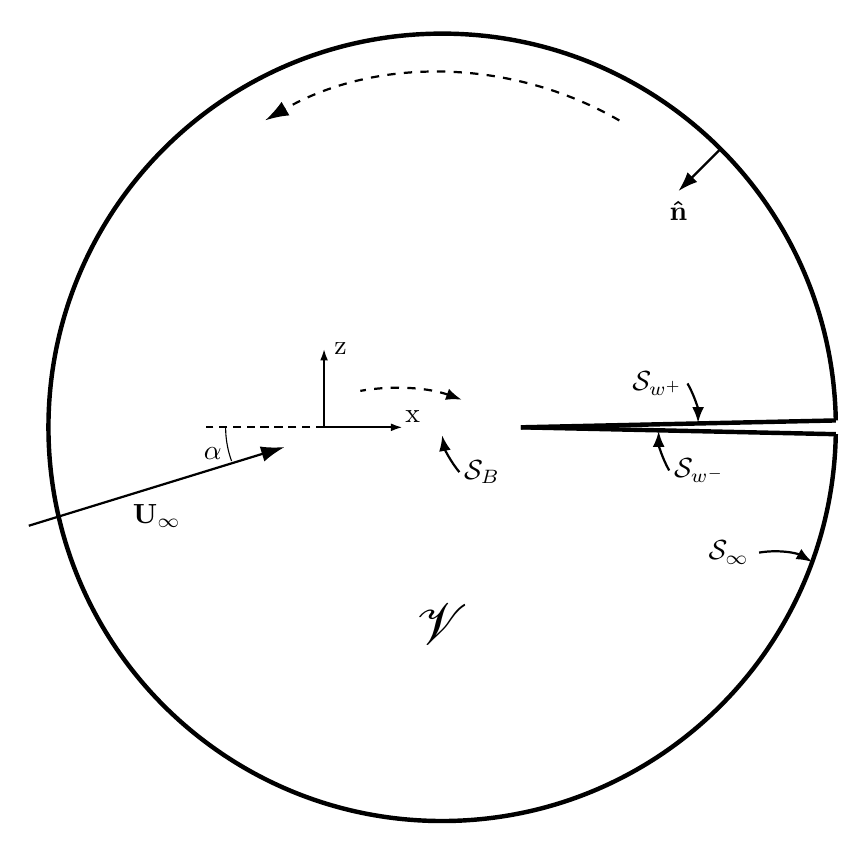
\begin{tikzpicture}
		%Circle
		\draw[ultra thick] (4.999,0.08726) arc (1:359:5);
		%Cut
		\draw[ultra thick] (1,0) -- (4.999,0.08726);
		\draw[ultra thick] (1,0) -- (4.999,-0.08726);
		%Axes
		\draw[thick,-{Latex[length=1.5mm,width=1mm]}] (-1.5,0) -- (-0.5,0) node[anchor=south west,yshift=-0.75mm,xshift=-1mm] {x};
		\draw[thick,-{Latex[length=1.5mm,width=1mm]}] (-1.5,0) -- (-1.5,1) node[anchor=west] {z};
		\draw[thick, densely dashed] (-1.5,0) -- (-3,0);
		%U infinity
		\draw[thick,-{Latex[length=3mm,width=2mm]}] (-5.25,-1.25) -- node[below,yshift=-1mm] {$\mathbf{U}_{\infty}$} (-2,-0.25);
		%aoa angle and label
		\draw (-2.75,0.0) arc (180:200:1.25) node[anchor=south east, yshift=-1mm] {$\alpha$};
		%Normal
		\draw[thick,-{Latex[length=2.5mm,width=1.75mm]}] (3.5355,3.5355) -- (3,3) node[below] {$\mathbf{\hat{n}}$};
		%outer boundary orientation
		\draw[thick,dashed,-{Latex[length=3mm,width=2mm]}] (2.25,3.897) arc (60:120:4.5cm);
		%Airfoil
		\draw[ultra thick] plot[smooth] file{figures/airfoil.dat};
		%body boundary orientation
		\draw[thick,dashed,{Latex[length=2mm,width=1.5mm]}-] (0.25,0.35) arc (70:100:2.5cm);
		%body boundary label
		\draw[thick,{Latex[length=2mm,width=1.5mm]}-] (0.0,-0.1) arc (190:220:1) node[anchor=west,xshift=-2] {$\mathcal{S}_{B}$};
		%upper wake boundary label
		\draw[thick,{Latex[length=2mm,width=1.5mm]}-] (3.25,0.0567) arc (0:30:1) node[anchor=east,xshift=2] {$\mathcal{S}_{w^+}$};
		%lower wake boundary label
		\draw[thick,{Latex[length=2mm,width=1.5mm]}-] (2.74958,-0.04799) arc (180:210:1) node[anchor=west,xshift=-2] {$\mathcal{S}_{w^-}$};
		%outer boundary label
		\draw[thick,{Latex[length=2mm,width=1.5mm]}-] (4.69846310393,-1.71010071663) arc (60:100:1) node[anchor=east] {$\mathcal{S}_{\infty}$};
		\draw (0.0,-2.5) node {\huge$\mathscr{V}$};
		\end{tikzpicture}
		\caption{Definition of problem boundaries. The dashed arrows indicate the boundary orientation. Note that the normal vector, $\mathbf{n}$, is directed \emph{into} the control volume.}
		\label{fig:boundarydef}
	\end{figure}
	
	
	Next we define the boundary value problem where, for any point, \(\mathbf{P}= [x,z]^T\) in \( \mathscr{V} \), the potential, \( \Phi(\mathbf{P}) \) is the solution to the boundary value problem:
	
	\begin{align}
	\label{eqn:2dlaplace}
	\nabla^2 \Phi(\mathbf{P}) = 0&, ~~~~\mathbf{P} \in \mathscr{V}\\ 
	\frac{\partial \Phi(\mathbf{P})}{\partial n}=0&, ~~~~\mathbf{P} \in \mathcal{S}_B\\
	\label{eqn:perturbpot}
	\Phi(\mathbf{P}) - \Phi_{\infty}(\mathbf{P}) \rightarrow 0&, ~~~~||\mathbf{P}||^2 \rightarrow \infty 
	\end{align}
	
	\noindent where at the infinite boundary \( \mathcal{S}_{\infty} \), the flow field is defined to be \( \nabla \Phi_{\infty} = \mathbf{U}_{\infty} = [u_{\infty}, w_{\infty}]^T\), and \( \Phi_{\infty}(\mathbf{P}) = \mathbf{U}_{\infty} \cdot \mathbf{P} = u_{\infty}x + w_{\infty}z\).
	
	
	We then apply Green's second identity with the perturbation potential from \cref{eqn:perturbpot}, that is, \( \phi(\mathbf{P}) = \Phi(\mathbf{P}) - \Phi_{\infty}(\mathbf{P}) \) and \( G(\mathbf{P},\mathbf{Q}) = (1/2\pi)\ln||\mathbf{P}-\mathbf{Q}|| \) (another solution to \cref{eqn:2dlaplace}, the two-dimensional Laplace equation). Doing so, we reformulate the boundary value problem as follows: 
	
	We begin with Green's second identity as stated in equation (8-9) in chapter 8 of Moran \cite{moran1984}, making a few alterations in variable names for consistency with this paper
	
	\begin{equation}
	\phi_P = \int_{\mathcal{S}_B + \mathcal{S}_W} \left[ \left( \mathbf{\hat{n}} \cdot \nabla \phi_Q \right) G - \phi_Q \left( \mathbf{\hat{n}} \cdot \nabla G \right) \right] \mathrm{d} \mathcal{S}
	\end{equation}
	
	\noindent where, \(\phi_P\) and \(\phi_Q\) are $\phi(\mathbf{P})$ and $\phi(\mathbf{Q})$ used in \cref{ssec:probform}. That is, the perturbation potentials associated with the field point $\mathbf{P}$ and the source point $\mathbf{Q}$, respectively. Likewise $G$ is $G(\mathbf{P},\mathbf{Q})$, another solution to the Laplace equation 
	
	\begin{align}
	G &= \frac{\ln{r}}{2\pi}~~~~\text{(in 2-D)}\\
	r &= |P-Q|
	\end{align}
	
	
	
	We do not include \(\mathcal{S}_{\infty}\) in the integral due to our use of the perturbation potential, which causes this portion of the integral to vanish.\cite{moran1984} 
	
	We now separate the integral into an integral over the body surface, and wake surface
	
	\begin{equation}
	\phi_P = \int_{\mathcal{S}_B} \left( \mathbf{\hat{n}} \cdot \nabla \phi_Q \right) G - \phi_Q \left( \mathbf{\hat{n}} \cdot \nabla G \right) \mathrm{d} \mathcal{S}_B + \int_{\mathcal{S}_W} \left( \mathbf{\hat{n}} \cdot \nabla \phi_Q \right) G - \phi_Q \left( \mathbf{\hat{n}} \cdot \nabla G \right) \mathrm{d} \mathcal{S}_W
	\end{equation}
	
	We defined the control volume such that the potential was twice differentiable throughout. We can see, however, that the potential is not continuous across \( \mathcal{S}_w \). Fortunately, the normal velocity and pressure are.
	
	\begin{align}
	\label{eqn:velocitycontinuity}
	\frac{\partial \Phi^+}{\partial n} &= \frac{\partial \Phi^-}{\partial n}~~~~\mathbf{P} \in \mathcal{S}_w\\
	p^+ &= p^-~~~~~~~~\mathbf{P} \in \mathcal{S}_w
	\end{align}
	
	Applying \cref{eqn:velocitycontinuity} and remembering that the normal vectors on either side of \( \mathcal{S}_w \) are directly opposite, we can simplify by taking the integral over both sides of \( \mathcal{S}_w \) simultaneously, causing the \(\mathbf{\hat{n}} \cdot \nabla \phi_Q\) term to cancel.  We can further simplify by assuming that the jump in $\phi$ across the wake is a constant (\( \Gamma = \phi^+_Q - \phi^-_Q = \mathrm{const}, ~\mathbf{Q} \in \mathcal{S}_w \)) and bring that outside of the integral leaving us with
	
	\begin{equation}
	\phi_P = \int_{\mathcal{S}_B} \left( \mathbf{\hat{n}} \cdot \nabla \phi_Q \right) G - \phi_Q \left( \mathbf{\hat{n}} \cdot \nabla G \right) \mathrm{d} \mathcal{S}_B + \Gamma \int_{\mathcal{S}_W} \left( \mathbf{\hat{n}} \cdot \nabla G \right) \mathrm{d} \mathcal{S}_W
	\end{equation}
	
	We then remember that there can be no flow through the solid body, or mathematically
	
	\begin{equation}
	\mathbf{\hat{n}} \cdot \nabla \Phi = 0
	\end{equation}
	
	\noindent but in our case we have defined $\phi$ to be the perturbation potential such that
	
	\begin{equation}
	\mathbf{U} = \mathbf{U_\infty} + \nabla \phi
	\end{equation}
	
	\noindent so that our boundary condition is actually mathematically described as
	
	\begin{equation}
	\mathbf{\hat{n}} \cdot \nabla \phi = -\mathbf{\hat{n}} \cdot U_{\infty}
	\end{equation}
	
	\noindent substituting this in and reorganizing leaves us with
	
	\begin{equation}
	\phi_P + \int_{\mathcal{S}_B} \phi_Q \left( \mathbf{\hat{n}} \cdot \nabla G \right) \mathrm{d} \mathcal{S}_B + \Gamma \int_{\mathcal{S}_W} \left( \mathbf{\hat{n}} \cdot \nabla G \right) \mathrm{d} \mathcal{S}_W = -\int_{\mathcal{S}_B} \left( \mathbf{\hat{n}} \cdot U_{\infty} \right) G \mathrm{d} \mathcal{S}_B
	\end{equation}
	
	Expressing the directional derivatives, \(\mathbf{\hat{n}} \cdot \nabla G \), with respect to the point $\mathbf{Q}$, leaves us with 
	
	\begin{equation}
	\begin{aligned}
	\label{eqn:continuousformulation}
	\phi(\mathbf{P})~+ &\int_{\mathcal{S}_B} \phi(\mathbf{Q})\frac{\partial G(\mathbf{P},\mathbf{Q})}{\partial n_Q} ds_Q + \Gamma \int_{\mathcal{S}_w} \frac{\partial G (\mathbf{P},\mathbf{Q})}{\partial n_Q} ds_Q =\\
	&- \int_{\mathcal{S}_B} \left(\mathbf{\hat{n}}(\mathbf{Q}) \cdot  \mathbf{U}_{\infty} \right) G(\mathbf{P},\mathbf{Q}) ds_Q~, ~~~\mathbf{P} \in \mathcal{S}_B
	% \textbackslash \mathbf{P}_{TE}
	\end{aligned}
	\end{equation}
	
	\noindent where $\mathbf{P}$ is a field point, $\mathbf{Q}$ is a source point, the subscript \(Q\) indicates an operation with respect to the point \(Q\), and $\Gamma$ is defined as
	
	\begin{equation} 
	\Gamma = \Phi^+(\mathbf{Q}) - \Phi^-(\mathbf{Q}) = \mathrm{const}, ~\mathbf{Q} \in \mathcal{S}_w 
	\end{equation} 
	
	\noindent in other words, the jump in potential across $\mathcal{S}_w$, which we assume to be constant along $\mathcal{S}_w$.
	
	%\begin{figure}[h!]
	%	\centering
	%	\includegraphics[draft,width=2in]{draft}
	%	\caption{Figure showing P and Q interaction. Show full plain airfoil, with a collocation point with a source point, and a highlighted element with the integration points distributed thereon. Label them appropriately }
	%	\label{fig:potentialdist}
	%\end{figure}
	%
	%\begin{figure}[h!]
	%	\centering
	%	\includegraphics[draft,width=2in]{draft}
	%	\caption{Figure showing the potential jump across the wake. Show trailing edge up to element of interest. label angle definitions.}
	%	\label{fig:potentialjump}
	%\end{figure}
	
	Additionally, we consider $\mathcal{S}_w$ to be a straight line extending from the trailing edge of the airfoil, as depicted in \cref{fig:boundarydef}, to infinity. Doing so, we can take the integral over the surface $\mathcal{S}_w$ to be
	
	\begin{equation}
	\label{eqn:wakeintegral}
	\int_{x_{TE}}^{\infty} \frac{\partial G (\mathbf{P},\mathbf{Q})}{\partial n_Q} ds_Q = \frac{1}{2\pi} \arctan\left( \frac{y_{\mathbf{P}} - y_{TE}}{x_{\mathbf{P}}-x_{TE}} \right)
	\end{equation}
	
	
	\subsubsection{Non-Uniform Rational Basis Splines}
	\label{sssec:nurbs}
	Before moving on to the discrete formulation in \cref{sssec:discform}, we take a moment to review some basic concepts of Non-Uniform Rational Basis Splines (NURBS) that will be important to understanding the discrete formulation and numerical implementations of the IgBEM. There is significant literature explaining NURBS, so our review here is brief. ``The NURBS Book'' by Piegl and Tiller is an excellent resource for detailed information on NURBS.\cite{Piegl1997The-NURBS-Book}
	
	We begin with the general equation of a NURBS curve
	\begin{equation}
	\mathbf{c}(t) = \sum_{i=0}^n R_{i,p}(t) \mathbf{d}_i ~~~t\in T = [k_{p-1},k_{n+1}]
	\end{equation}
	
	\noindent where $\mathbf{c}(t)$ are the points along the NURBS curve, $[x(t),z(t)]$, located at parametric locations, $t$. The parametric points, $t$, lie within the range of knots, $k$ over which the spline is defined. In our case, the knots defining the spline are in the range $[0,1]$ and make up the knot vector $\mathbf{\mathcal{K}} = [k_0,k_1,\ldots,k_{n+p}]$ , and are in non-decreasing order. $R_{i,p}(t)$ are the rational B-Spline basis functions of degree $p$ defined over the range of $\mathcal{K}$, with non-negative weights, $\mathbf{w}$. $\mathbf{d}_i$ are the control points associated with each basis function, and make up a two-dimensional vector including, in our case, $x$ and $z$ coordinates. See \cref{ssec:airfoilparam} for details on how we apply NURBS in airfoil geometry definition.
	
	
	\subsubsection{Discrete Formulation}
	\label{sssec:discform}
	%\emph{Note: need to implement desingularized scheme.  (need to ask Dr. Scott about that vs. his weakly singular stuff first though. It may be better to do it his way than the other way.) Thereby removing integration issues, getting better convergence, and removing all the bad stuff in general.}
	
	As with the continuous formulation, the discrete formulation is also well documented,\cite{Politis2014, Kostas2017Shape-optimizat} but we repeat it here for ease of reference. We begin constructing the discrete problem formulation by applying the NURBS definition to the elements of \cref{eqn:continuousformulation}, putting the points $\mathbf{P}$ and $\mathbf{Q}$ in terms of a NURBS curve, associated with knots, $t$ and $\tau$, in the knot vector, $T$ (that is to say, $t$ and $\tau$ are both parametric locations within the range of the knot vector , $T$), such that
	
	\begin{equation}
	\begin{aligned}
	\mathbf{P} &= \mathbf{c}(t)\\
	\mathbf{Q} &= \mathbf{c}(\tau)\\
	\end{aligned}
	\end{equation}
	
	This constitutes a change of basis, so we will need to multiply by the jacobian of transformation, \(J(\tau) = ||\dot{\mathbf{c}}(\tau)||\). Including these modifications, along with \cref{eqn:wakeintegral} we write \cref{eqn:continuousformulation} as
	
	\begin{equation}
	\begin{aligned}
	\label{eqn:discreteformulationlong}
	\phi(\mathbf{c}(t))~+ &\int_{T} \phi(\mathbf{c}(\tau))\frac{\partial G(\mathbf{c}(t),\mathbf{c}(\tau))}{\partial n_\tau} J(\tau) d\tau +  \frac{\Gamma}{2\pi} \arctan\left( \frac{y_{\mathbf{P}} - y_{TE}}{x_{\mathbf{P}}-x_{TE}} \right) =\\
	&- \int_{T} \left(\mathbf{\hat{n}}(\mathbf{c}(\tau)) \cdot  \mathbf{U}_{\infty} \right) G(\mathbf{c}(t),\mathbf{c}(\tau))J(\tau) d\tau~, ~~~\mathbf{t} \in (0,1)
	\end{aligned}
	\end{equation}
	
	\noindent In order to simplify the notation, we define the following
	\begin{equation}
	\centering
	\begin{aligned}
	\label{eqn:simplenotation}
	\phi(t) &\equiv \phi(\mathbf{c}(t))\\
	\phi(\tau) &\equiv \phi(\mathbf{c}(\tau))\\
	K(t,\tau) &\equiv \frac{\partial G(\mathbf{c}(t),\mathbf{c}(\tau))}{\partial n_\tau}J(\tau)\\
	g(t) &\equiv -\int_{T} \left(\mathbf{\hat{n}}(\mathbf{c}(\tau)) \cdot  \mathbf{U}_{\infty} \right) G(\mathbf{c}(t),\mathbf{c}(\tau))J(\tau) d\tau \\
	\end{aligned}
	\end{equation}
	
	\noindent Rewriting with this simplified notation gives us
	
	\begin{equation}
	\label{eqn:discreteformulation}
	\phi(t) + \int_{T} \phi(\tau) K(t,\tau) d\tau + \frac{\Gamma}{2\pi} \arctan\left( \frac{y(t) - y_{TE}}{x(t)-x_{TE}} \right) = g(t), ~~~\mathbf{t} \in (0,1)
	\end{equation}
	
	\noindent The kernel $K(t,\tau)$ can be expressed as
	
	\begin{equation}
	\begin{aligned}
	K(t,\tau) &= \frac{ \dot{\mathbf{c}}(\tau) \wedge \left( \mathbf{c}(t) - \mathbf{c}(\tau) \right) }{2\pi||\mathbf{c}(t)-\mathbf{c}(\tau)||^2} &~~~\mathrm{if}~~~ t\neq\tau\\
	K(t,t) &= \frac{\dot{\mathbf{c}}(t)\wedge\ddot{\mathbf{c}}(t) }{2\pi||\dot{\mathbf{c}}(t)||^2} &~~~\mathrm{if}~~~  t=\tau
	\end{aligned}
	\end{equation}
	
	\noindent where `$\wedge$' indicates a two-dimensional exterior product. If we expand and put things in terms of $x$ and $z$ we get
	
	\begin{equation}
	\begin{aligned}
	K(t,\tau) &= \frac{ \dot{x}(\tau) \left[ z(t) - z(\tau) \right] - \dot{z}(\tau) \left[ x(t) - x(\tau) \right] }{2\pi\left( \left[ x(t) - x(\tau) \right]^2 + \left[ z(t) - z(\tau) \right]^2 \right)}  &~~~\mathrm{if}~~~ t\neq\tau\\
	K(t,t) &= \frac{ \dot{x}(t)\ddot{z}(t) - \dot{z}(t)\ddot{x}(t) }{2\pi\left( \dot{x}(t)^2  + \dot{z}(t)^2 \right)} &~~~\mathrm{if}~~~  t=\tau
	\end{aligned}
	\end{equation}
	
	We next project the perturbation potential, \( \phi(t) \), onto the same spline space 
	
	\begin{equation}
	\label{eqn:projection}
	\phi(t) = \sum_{i=0}^{n}\varphi_i R_{i,p}(t),~~~t \in [k_0,k_{n+p}]
	\end{equation}
	
	\noindent where \(R_{i,p}\) are the same bases used to define the geometry and \(\varphi\) are the set of unknowns for which we want to solve in order to characterize the potential distribution about the airfoil. $\varphi$ are analogous to the control points defining the geometry. 
	
	Often we will want to refine things beyond what the given geometry can offer in order to achieve an accurate solution. We can do this through a knot insertion process, which, by definition, does not alter the spline space onto which we are projecting. After properly refining through knot insertion, we should alter our expression in \cref{eqn:projection} for clarity. We express the refined perturbation potential as
	
	\begin{equation}
	\label{eqn:refinedprojection}
	\phi(t) = \sum_{i=0}^{n+m}\varphi_i R_{i,p}^{(m)}(t),~~~t \in T
	\end{equation}
	
	\noindent where $R_{i,p}^{(m)}$ are the adjusted bases after the knot insertion ($R_{i,p}^{(0)} \equiv R_{i,p}$ from \cref{eqn:projection}), and $m$ is the number of knots we inserted into the knot vector, $\mathcal{K}$, as part of our refinement. \Cref{fig:refinedmesh} shows graphically the knot insertion process.
	
	With this projection, we express \cref{eqn:discreteformulation} as
	
	\begin{equation}
	\label{eqn:discrete1}
	\sum_{i=0}^{n+m}\varphi_i R_{i,p}^{(m)}(t) + \int_{T} \sum_{i=0}^{n+m}\varphi_i R_{i,p}^{(m)}(\tau) K(t,\tau) d\tau + \frac{\Gamma}{2\pi} \arctan\left( \frac{y(t) - y_{TE}}{x(t)-x_{TE}} \right) = g(t)
	\end{equation}
	
	\noindent At this point we should also note that the bases only need be integrated over the ranges where they are non-zero. To this end, we define our projection of \(\phi(t)\) on each element to be
	
	\begin{equation}
	\label{eqn:elementprojection}
	\phi(t) = \sum_{\ell=1}^{p+1}\varphi^{\ell e} N_{\ell}^{e}(t)
	\end{equation}
	
	\noindent which is equivalent to \cref{eqn:refinedprojection} such that \(N_{\ell}^{e}(t)\) is the \(\ell\)-th non-zero basis function, \(R_{i,p}^{(m)}(t)\), on element $e$, and \(\varphi^{\ell e}\) is the \(\varphi_i\) associated with that basis function.
	
	We now want to define a local coordinate system on each element, \(\hat{\tau} = [-1,1]\). This allows for simple numerical integration across elements. By transforming our coordinates again, we will again need to apply a Jacobian of transformation, \(J(\hat{\tau}) = \text{d}\tau/\text{d}\hat{\tau} \).
	
	As a final step, we define the points $t$ in \cref{eqn:discrete1} to be the Greville abscissae, \(\xi\), of the knot vector, defined as
	
	\begin{equation}
	\label{eqn:grevilleabscissae}
	\xi_j = \frac{1}{p}\left(k_{j+1} + k_{j+2} + \dots + k_{j+p-1} \right)
	\end{equation}
	
	\noindent Applying \cref{eqn:grevilleabscissae,eqn:elementprojection} to \cref{eqn:discrete1}, we obtain the following system of equations.
	
	\begin{equation}
	\sum_{\ell=1}^{p+1}\varphi^{\ell e} N_{\ell}^{e}(\xi_j) +  \sum_{e=1}^{N_e} \sum_{\ell=1}^{p+1} \left[ \varphi^{\ell e} \int_{-1}^{1} N_{\ell}^{e}(\hat{\tau}) K(\xi_j,\hat{\tau}) J(\hat{\tau}) d\hat{\tau} \right] + \frac{\left(\varphi_n - \varphi_0 \right)}{2\pi} \arctan\left( \frac{y(\xi_j) - y_{TE}}{x(\xi_j)-x_{TE}} \right) = g(\xi_j)
	\end{equation}
	
	\noindent with which we can solve for the unknown $\varphi$, and thus $\phi$, anywhere on $\mathcal{S}_B$.
	
	%\begin{equation}
	%	\begin{bmatrix}
	%	x       & x & x & \dots & x \\
	%	x       & x & x & \dots & x \\
	%	\hdotsfor{5} \\
	%	x       & x & x & \dots & x
	%	\end{bmatrix}
	%	\begin{bmatrix}
	%	\varphi_0    \\
	%	\varphi_1    \\
	%	\vdots \\
	%	\varphi_n       
	%	\end{bmatrix}
	%	=
	%	\begin{bmatrix}
	%	g(\xi_0) \\
	%	g(\xi_1) \\
	%	\vdots \\
	%	g(\xi_n)
	%	\end{bmatrix}
	%\end{equation}
	
	\subsubsection{Obtaining Velocity and Pressure Fields}
	
	The coefficient of pressure, \(c_{\mathrm{P}}\), can be computed as
	\begin{equation}
	c_{\mathrm{P}} = 1 - \frac{v_{\mathrm{tan}}^2}{|\mathbf{U}_{\infty}|^2}
	\end{equation}
	
	\noindent where \(v_{\mathrm{tan}}\) is the tangential velocity, and is defined at any parametric point, \(t \in T\), as
	
	\begin{equation}
	v_{\mathrm{tan}} = \mathbf{U}_{\infty} \cdot \hat{\mathbf{t}} + \frac{\partial \phi}{\partial s} = \mathbf{U}_{\infty} \cdot \hat{\mathbf{t}} + \sum_{i=0}^{n} \varphi_i \frac{d R_{i,p}(t)}{dt} \frac{1}{||\dot{\mathbf{c}}(t)||}
	\end{equation}
	
	\noindent where $\hat{\mathbf{t}}$ is the unit tangent vector on the airfoil surface at point $t$.
	
	\subsection{Airfoil Parameterization}
	\label{ssec:airfoilparam}
	
	Because the analysis above is based in NURBS, we need a parameterization method based in NURBS. Rajnarayan et. al. proposed a parameterization method, here we review it. This parameterization method uses three inputs to define the control points: nose radius ($r_{LE}$), trailing-edge half thickness ($\Delta z_{TE}$), and boat-tail angle ($\beta_{TE}$). In addition to these parameters, we included the angle of the camber line ($\gamma$) so we had the ability to approximate airfoils with camber. When we approximated airfoils, we let $z_{TE}$ equal zero.
	
	In order to create a boundary that is a $C^2$ continuous curve, we used a cubic NURBS curve that spanned 7 control points. (Opportunity to talk about why we need a continuous boundary.) The (X,Y) location of the seven control points of the NURBS curve "that satisfy terminal constraints on airfoil shape" are defined as follows: 
	
	
	\begin{equation}
	\renewcommand\arraystretch{1.5}
	\begin{bmatrix}
	P_1 \\ 
	P_2 \\
	P_3 \\
	P_4 \\
	P_5 \\
	P_6 \\
	P_7
	\end{bmatrix}
	=
	\begin{bmatrix}
	1 & 0 \\ 
	\nicefrac{1}{3} & \Delta z_{TE}+\frac{2}{3}\tan(\gamma-\beta_{TE})  \\ 
	0 & -\frac{1}{3}(2r_{LE})^{\nicefrac{1}{2}} \\
	0 & 0 \\
	0 & \frac{1}{3} (2r_{LE})^{\nicefrac{1}{2}}\\
	\nicefrac{1}{3} & \Delta z_{TE}+\frac{2}{3}\tan(\gamma+\beta_{TE}) \\
	1 & \Delta z_{TE}
	\end{bmatrix} 
	\end{equation}
	
	%\begin{figure}[h!]
	%	\centering
	%	\includegraphics[draft,width=2in]{draft}
	%	\caption{ADAM's FIGURE: Figure showing various parameter's on an arbitrary airfoil}
	%	\label{fig:airfoilparam}
	%\end{figure}
	
	
	\section{Introduction}
	
	
	
	
	\bigskip
	
	\bibliographystyle{aiaa} 
	\bibliography{igapanel.bib}{}
	
	
\end{document}